\documentclass[border=0.2cm]{standalone}

\usepackage{tikz}
\usetikzlibrary{shapes.geometric, shapes.misc}
\usetikzlibrary{cd, fit, calc}
\usetikzlibrary{positioning}
\usetikzlibrary{decorations.markings}

\tikzset{middlearrow/.style={
        decoration={markings,
            mark= at position .5 with {\arrow{#1}} ,
        },
        postaction={decorate}
    }
}

\begin{document}

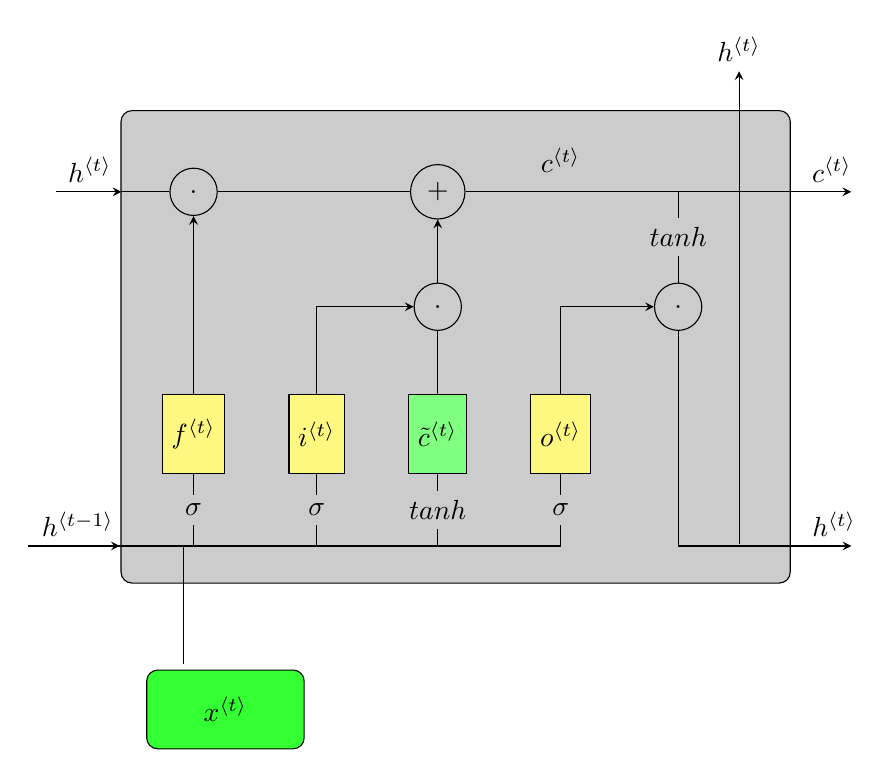
\begin{tikzpicture}

\node[rounded corners, draw, inner xsep = 3mm, inner ysep=1cm, fill=black!20, minimum width=8.5cm,minimum height=6cm] (largerec) at(-.5,0){};

\matrix[row sep=0.8cm,column sep=0.8cm] {
    \node [draw, circle, minimum size=.6cm] (circle1) { . }; &
    &
    \node [draw, circle, minimum size=.6cm] (circle2) { + }; &
    \node [label={$ c ^{\langle{} t \rangle{} } $}] (hid) { }; &
    \node [] (hid) { }; &
    \\
    &
    &
    \node [draw, circle, minimum size=.6cm] (circle3) { . }; &
    &
    \node [draw, circle, minimum size=.6cm] (circle4) { . }; &
    \\
    \node (rect) [draw, fill=yellow!50, minimum width=.6cm,minimum height=1cm] (rect1) { {$ f ^{\langle{} t \rangle{} } $ }}; &
    \node (rect) [draw, fill=yellow!50, minimum width=.6cm,minimum height=1cm] (rect2) { {$ i ^{\langle{} t \rangle{} } $ }}; &
    \node (rect) [draw, fill=green!50, minimum width=.6cm,minimum height=1cm] (rect3) { {$ \tilde c ^{\langle{} t \rangle{} } $ }}; &
    \node (rect) [draw, fill=yellow!50, minimum width=.6cm,minimum height=1cm] (rect4) { {$ o ^{\langle{} t \rangle{} } $ }}; &
    &
    \\
    \node [] (hid1) { }; &
    \node [] (hid2) { }; &
    \node [] (hid3) { }; &
    \node [] (hid4) { }; &
    \node [] (hid5) { }; &
    &
    \\
    };

\node [rounded corners, draw, fill=green!80, minimum width=2cm, minimum height=1cm] at ($(rect1.east)+(0,-3.5)$)(rect5)  {$ x ^{\langle{} t \rangle{} } $};

\draw [-stealth] (rect1.north) -- (circle1.south) {};
\draw [-stealth] (circle3.north) -- (circle2.south) {};
\draw [] (circle1.east) -- (circle2.west) {};
\draw [] (rect3.north) -- (circle3.south) {};
\draw[-stealth, to path={|- (\tikztotarget)}] (rect2) edge (circle3);
\draw[-stealth, to path={|- (\tikztotarget)}] (rect4) edge (circle4);

\path[draw,-] (hid.center) -- (circle4) node[midway,anchor=center, fill=black!20] {$tanh$};
\path[draw,-] (rect4) -- (hid4.center) node[midway,anchor=center, fill=black!20] {$\sigma$};
\path[draw,-] (rect3) -- (hid3.center) node[midway,anchor=center, fill=black!20] {$tanh$};
\path[draw,-] (rect2) -- (hid2.center) node[midway,anchor=center, fill=black!20] {$\sigma$};
\path[draw,-] (rect1) -- (hid1.center) node[midway,anchor=center, fill=black!20] {$\sigma$};
\path[draw,-] (circle4) -- (hid5.center) node[] {};

\draw[middlearrow={stealth reversed}] (circle1) -- node[pos=.7, above] {$ h ^{\langle{} t \rangle{} } $} ++(-1.75,0);
\draw [-stealth, align=right] (circle2) -- node[ above, pos=.95] {$ c ^{\langle{} t \rangle{} } $} ++(5.25,0);
\draw [middlearrow={stealth reversed}] (hid1.center) -- node[ above, pos=.7] {$ h ^{\langle{} t-1 \rangle{} } $} ++(-2.1,0);
\draw [] (hid1.center) -- (hid4.center) {};

\draw[-stealth] (hid5.center) -- node[pos=.9, above] {$ h ^{\langle{} t \rangle{} } $} ++(2.2,0);
\draw[] (hid1.west) -- ++(0,-1.5){};
\draw[-stealth] (3.1,-2.5) -- node[pos=1, above] {$ h ^{\langle{} t \rangle{} } $} ++(0,6);

\end{tikzpicture}
\end{document}